\chapter{Current peak transducer}
\section{Theory and related work} \label{sec:literature_current_peak_transducer}
The design for the current peak transducer consisted of a current sense resistor in series with the load, a non inverting operational amplifier gain stage, and a precision rectifier transducer implemented as in Section \ref{sec:design_voltage_peak_transducer}. A current sense resistor is a resistor placed in series with a load to allow current to be measured, the voltage across the resistor will be directly proportional to the current being measured. A non inverting amplifier is an operational amplifier configuration where the input voltage signal is connected to the non-inverting input to the operational amplifier. The feedback control consists of a resistor divider network that connects the output to the inverting input, this resistor divider network sets the gain of the amplifier, produces a good stability and has a high input impedance \ref{yourmom}. 
%https://www.electronics-tutorials.ws/opamp/opamp_3.html

\section{Design} \label{sec:design_current_peak_transducer}
The first part of this design included a sense resistor which was added in series with the load to turn a current measurement into a voltage measurement, this voltage measurement was then amplified to a suitable voltage level usable by the peak transducer. For the purpose of this design a $\SI{30}{\milli \Omega}$ sense resistor was chosen to ensure a reasonable trade off between power losses in the system and the measured voltage level over the sense resistor. It was found that a smaller sense resistor would by Ohm's law have a smaller voltage drop over it, and this in return would require a larger voltage gain stage, which was not desirable as such a large gain would require a very large feedback resistor, with a very large deviation from its given resistance. It was chosen that the current peak transducer would be able to measure a maximum current of \SI{350}{\milli A}, this corresponded to a sense voltage of \SI{10.5}{\milli V}.\newline
Given that the Arduino's maximum pin voltage was given as \SI{5}{\volt}, and to ensure a maximum resolution for the \SI{350}{\milli A} measurement range, the \SI{10.5}{\milli V} maximum sense voltage had to be amplified using an operational amplifier. This operational amplifier configuration was chosen as a differential mode non-inverting amplifier utilizing both the \SI{5}{\volt} and the \SI{-5}{\volt} rails as its power supplies. It was found that the maximum input to any of the operational amplifiers pins was not to exceed \SI{5}{\volt} or \SI{-5.3}{\volt} \ref{yourmom}.
The desired gain, and ratio between input resistor $R_1$, and feedback resistor $R_2$ was calculated by using Equation \ref{eq:opampgain}. Here $R_1$ was chosen as $\SI{1}{\kilo \Omega}$, and given this $R_2$ was found to be $\SI{470}{\kilo \Omega}$.\newline
\begin{align}
   \frac{V_{out}}{V_{in}}=1+\frac{R_2}{R_1}
   \label{eq:opampgain}
\end{align}
Given that the sense voltage was now amplified to a suitable range between 0 and \SI{5}{\volt} the same design procedure as Section \ref{sec:design_voltage_peak_transducer} could be applied to measure the amplitude of the peak of the sinusoidal input. This precision rectifier circuit utilised both the \SI{5}{\volt} and the \SI{-5}{\volt} rails as its power supplies, and thus it was not required that the negative half cycle of the sinusoidal input, with a maximum peak of \SI{5}{\volt}, be rectified as the minimum differential mode input to the operational amplifier was \SI{-5.3}{\volt}. A ripple voltage of no more than \SI{10}{\milli \volt} was chosen and from this the output capacitor to the peak detector was calculated in exactly the same way as in Section \ref{sec:design_voltage_peak_transducer} using Equation \ref{eq:ripplevoltage}, the desired capacitor value was found as $\SI{10}{\micro F}$.
Given the specification of a maximum load current of \SI{350}{\milli A} corresponding to a voltage of $\SI{5}{VAC}$ and the Arduino having a range of $4095$ bits, it can be calculated that the resolution of the ADC would be $\SI{85.47}{\micro A}$ per bit.
\begin{figure}[h!]
    \centering
    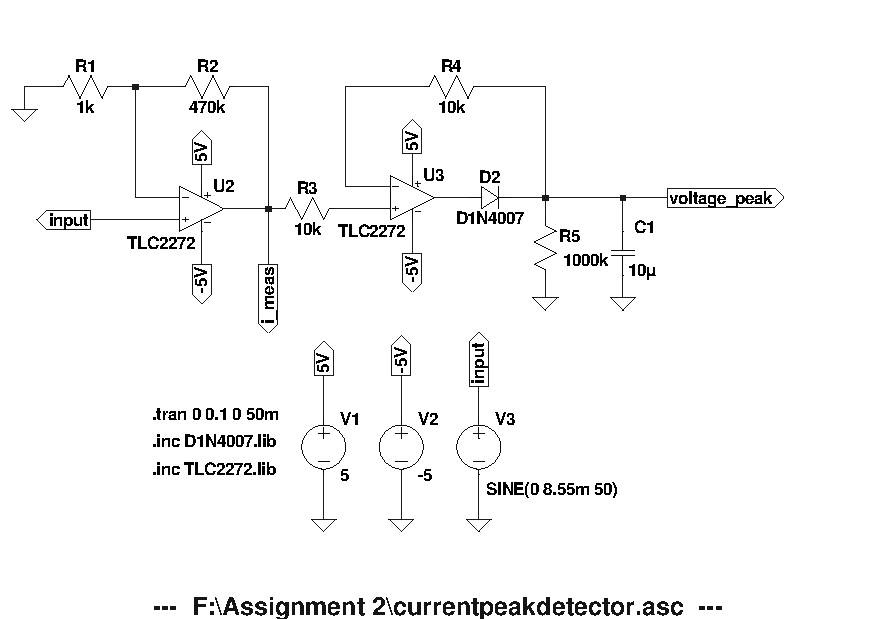
\includegraphics[width = 0.65\linewidth]{Figures/currentpeakdetector.pdf}
        \caption{Current Peak Transducer Diagram}
    \label{fig:currentpeakdetector.pdf}
\end{figure}

\section{Simulation} \label{sec:simulation_switchmode}

\section{Measurements} \label{sec:measurements_switchmode}








